\documentclass[11pt,a4paper]{article}

\usepackage[T1]{fontenc}
\usepackage[utf8]{inputenc}
\usepackage{lmodern}
\usepackage[a4paper,margin=24mm,headheight=15pt]{geometry}
\usepackage{microtype}
\usepackage{graphicx}
\usepackage{pdflscape}
\usepackage[table]{xcolor}
\usepackage{booktabs,tabularx,longtable,array}
\usepackage{enumitem,parskip,ragged2e}
\usepackage{amsmath,amssymb}
\usepackage{listings}
\usepackage{caption}
\usepackage{fancyhdr,titlesec}
\usepackage{hyperref}

\definecolor{Navy}{HTML}{173A66}
\definecolor{Blue}{HTML}{2F75B5}
\definecolor{Teal}{HTML}{008C8C}
\definecolor{Amber}{HTML}{C69214}
\definecolor{PaleBlue}{HTML}{EAF3FA}
\definecolor{PaleTeal}{HTML}{E8F6F4}
\definecolor{PaleAmber}{HTML}{FFF6DC}
\definecolor{SoftGray}{HTML}{F3F5F7}
\definecolor{RuleGray}{HTML}{CAD2DA}
\definecolor{DarkGray}{HTML}{3E4A55}

\hypersetup{
  colorlinks=true,
  linkcolor=Navy,
  urlcolor=Teal,
  citecolor=Navy,
  pdftitle={Dawid-Skene on the Server: Proposed Changes and Controlled Experiment Plan},
  pdfsubject={Plain-English design and feasibility report},
  pdfkeywords={Dawid-Skene, federated learning, pseudo-labels, server aggregation}
}

\graphicspath{{./}{../../}}
\setlength{\parindent}{0pt}
\setlength{\parskip}{0.55em}
\setlist[itemize]{leftmargin=1.45em,itemsep=0.25em,topsep=0.35em}
\setlist[enumerate]{leftmargin=1.65em,itemsep=0.3em,topsep=0.35em}
\renewcommand{\arraystretch}{1.18}
\setlength{\tabcolsep}{5pt}
\emergencystretch=3em

\newcolumntype{Y}{>{\RaggedRight\arraybackslash}X}
\newcolumntype{L}[1]{>{\RaggedRight\arraybackslash}p{#1}}

\titleformat{\section}
  {\Large\bfseries\color{Navy}}{\thesection}{0.65em}{}
\titleformat{\subsection}
  {\large\bfseries\color{Blue}}{\thesubsection}{0.65em}{}
\titleformat{\subsubsection}
  {\normalsize\bfseries\color{Teal}}{\thesubsubsection}{0.65em}{}
\titlespacing*{\section}{0pt}{2.0em}{0.65em}
\titlespacing*{\subsection}{0pt}{1.4em}{0.45em}

\pagestyle{fancy}
\fancyhf{}
\fancyhead[L]{\small\color{DarkGray}Dawid-Skene server aggregation}
\fancyhead[R]{\small\color{DarkGray}Plain-English change guide}
\fancyfoot[C]{\small\color{DarkGray}\thepage}
\renewcommand{\headrulewidth}{0.4pt}
\renewcommand{\footrulewidth}{0pt}

\lstdefinestyle{plainpseudo}{
  basicstyle=\ttfamily\small,
  backgroundcolor=\color{SoftGray},
  frame=single,
  rulecolor=\color{RuleGray},
  framerule=0.5pt,
  breaklines=true,
  columns=fullflexible,
  keepspaces=true,
  showstringspaces=false,
  xleftmargin=0.5em,
  xrightmargin=0.5em,
  aboveskip=0.7em,
  belowskip=0.7em
}

\newcommand{\code}[1]{\texttt{#1}}
\newcommand{\pp}{percentage points}

\begin{document}
\hypersetup{pageanchor=false}

\begin{titlepage}
  \thispagestyle{empty}
  \vspace*{18mm}

  {\color{Navy}\rule{\textwidth}{1.6pt}}\\[10mm]
  {\Huge\bfseries\color{Navy}Dawid-Skene on the Server\par}
  \vspace{4mm}
  {\LARGE\color{Blue}Proposed Changes and Controlled Experiment Plan\par}
  \vspace{8mm}
  {\Large A plain-English guide\par}

  \vspace{18mm}
  \begin{center}
    \setlength{\fboxsep}{12pt}
    \fcolorbox{Blue}{PaleBlue}{%
      \begin{minipage}{0.86\textwidth}
        \textbf{Document status:} design and feasibility plan only.\\[2mm]
        \textbf{Main conclusion:} the change is technically feasible as a server-only experiment,
        but it has not yet been implemented, validated, or approved as the default.\\[2mm]
        \textbf{Change boundary:} clients keep doing exactly what they do today. Dawid-Skene is
        added only where the server combines the clients' hard-label proposals.
      \end{minipage}}
  \end{center}

  \vfill
  \begin{tabular}{@{}ll@{}}
    \textbf{Branch:} & \code{dawid-skene} \\
    \textbf{Prepared:} & 11 August 2026 \\
    \textbf{Audience:} & researchers, engineers, reviewers, and non-specialist stakeholders \\
  \end{tabular}

  \vspace{12mm}
  {\color{Navy}\rule{\textwidth}{1.6pt}}
\end{titlepage}

\pagenumbering{roman}
\hypersetup{pageanchor=true}
\setcounter{tocdepth}{1}
\tableofcontents
\clearpage
\pagenumbering{arabic}

\section{Executive summary}

Today, every client gives the server a proposed class label for each sample in a shared open
dataset. A client can also abstain when it is not confident that a sample is familiar. The server
currently combines the submitted labels by counting votes.

The proposed change replaces only that vote-counting decision with Dawid-Skene server aggregation.
Dawid-Skene does more than count answers. It repeatedly estimates two things together:

\begin{itemize}
  \item the most likely true class of each shared sample; and
  \item the class-specific mistake pattern of each client that supplied enough labels.
\end{itemize}

This can help when clients have different strengths. For example, one client may distinguish two
traffic classes well while another often confuses them. Majority voting treats both opinions as
equally informative. Dawid-Skene can learn their different confusion patterns from the label table
and use those patterns when estimating the final label.

\begin{center}
  \setlength{\fboxsep}{10pt}
  \fcolorbox{Teal}{PaleTeal}{%
    \begin{minipage}{0.91\textwidth}
      \textbf{The most important boundary}\par
      Client training, client prediction, the discriminator, filtering, hard-label upload,
      distillation, the dataset, and the network payload remain unchanged. The new calculation is
      entirely inside the server's hard-label aggregation step. Supporting server configuration,
      diagnostics, reports, audits, and tests must also be added so the change can be run safely.
    \end{minipage}}
\end{center}

The recommended first use is \textbf{shadow mode}. In shadow mode, the server computes
Dawid-Skene and records what it would have decided, but still broadcasts the existing majority
result. This gives a safe comparison on exactly the same client submissions. Active use should
begin only after mathematical, accuracy, latency, privacy, and failure-handling gates pass.

This is a proposed adaptation of the Dawid-Skene idea, not a reproduction of the complete FedDS
method in the reference paper. The paper uses reliability estimates to weight uploaded model
parameters. This repository does not upload client models in this workflow. Here, Dawid-Skene is
used only to combine the hard pseudo-labels that clients already upload.

\section{The current workflow}

One current federated round can be understood in seven steps:

\begin{enumerate}
  \item Each client trains its persistent classifier on its own labelled data.
  \item The classifier predicts classes for the same shared open dataset.
  \item The client's discriminator decides which samples appear familiar enough to use.
  \item The client uploads a hard-label vector. Legal class values are 0 through 10. The value
        \code{-1} means ``I abstain for this sample.''
  \item The server checks the submissions and combines the labels by deterministic majority vote.
  \item The server broadcasts one \code{global\_labels} vector and one \code{valid\_mask} vector.
  \item Existing client distillation and server-model training consume those two arrays.
\end{enumerate}

All clients label the same ordered list of 8,900 open samples. This common ordering is what makes a
client-by-sample annotation table possible on the server.

\section{Exactly what changes}

\begin{table}[htbp]
\centering
\caption{Current and proposed server behavior.}
\begin{tabularx}{\textwidth}{L{0.21\textwidth}YY}
\toprule
\textbf{Area} & \textbf{Current behavior} & \textbf{Proposed behavior} \\
\midrule
Label aggregation & Count each accepted client label equally and choose the lowest class index if
there is an exact tie. & Estimate a class prior, one class-specific confusion matrix per eligible
client, and a posterior class probability per sample; then choose the most likely class. \\
Operating modes & Majority only. & Majority, shadow Dawid-Skene, or active Dawid-Skene. Majority
remains the software default. \\
Failure behavior & Use the majority result produced by the current path. & Return visibly and
deterministically to that majority result if Dawid-Skene lacks support, becomes numerically invalid,
or does not converge under the locked policy. \\
Diagnostics & Vote totals, participation, labels, and masks. & Add convergence, iterations,
objective history, raw likelihood, timing, disagreement, fallback reason, support, and restricted
client-confusion summaries. \\
Configuration & No Dawid-Skene fields. & Add explicit, validated options for initialization,
smoothing, evidence thresholds, stopping, numerical safety, fallback, and audit storage. \\
Reporting & Existing experiment identity. & Keep extension runs separate by run kind and aggregation
mode so they cannot replace a canonical report cell. \\
Testing & Existing majority and protocol tests. & Add mathematical, missing-data, determinism,
failure, privacy, resume, reporting, and performance tests. \\
\bottomrule
\end{tabularx}
\end{table}

\subsection{What does not change}

\begin{itemize}
  \item No client model parameters are uploaded.
  \item No client-side Dawid-Skene calculation is added.
  \item Clients keep training, predicting, filtering, and uploading the same hard-label vector.
  \item \code{-1} remains an abstention. It does not become a twelfth class.
  \item The uplink and downlink keep the same array names, shapes, data types, and logical byte
        counts. Serialized message sizes are measured separately because values can change.
  \item The server still broadcasts only \code{global\_labels} and \code{valid\_mask}. It never
        broadcasts posterior probabilities, confusion matrices, or reliability scores.
  \item Existing distillation and server-model training continue after the aggregation decision.
  \item The dataset, partitions, CNN backbone, optimizer, learning rate, local epochs, batch size,
        discriminator setting, and primary round count remain locked between experimental arms.
  \item True open-set labels remain unavailable to live aggregation and training.
\end{itemize}

\subsection{Notation used in the architecture}

The detailed figure on the next page uses the following short names:

\begin{tabularx}{\textwidth}{L{0.16\textwidth}Y}
\toprule
\textbf{Symbol} & \textbf{Plain-English meaning} \\
\midrule
$J$ & Number of accepted clients in the current server aggregation. \\
$N$ & Number of shared open samples; currently 8,900. \\
$C$ & Number of classes; currently 11. \\
$Y$ & The client-by-sample table of submitted labels. \\
$Q$ & The estimated probability of every candidate class for every usable sample. \\
$M_j$ & Client $j$'s estimated class-specific confusion matrix for this round. \\
$\pi$ & Estimated class proportions for the usable samples. \\
\code{-1} & Missing observation because the client abstained; never a class. \\
\bottomrule
\end{tabularx}

\clearpage
\begin{landscape}
\thispagestyle{fancy}
\begin{figure}[p]
  \centering
  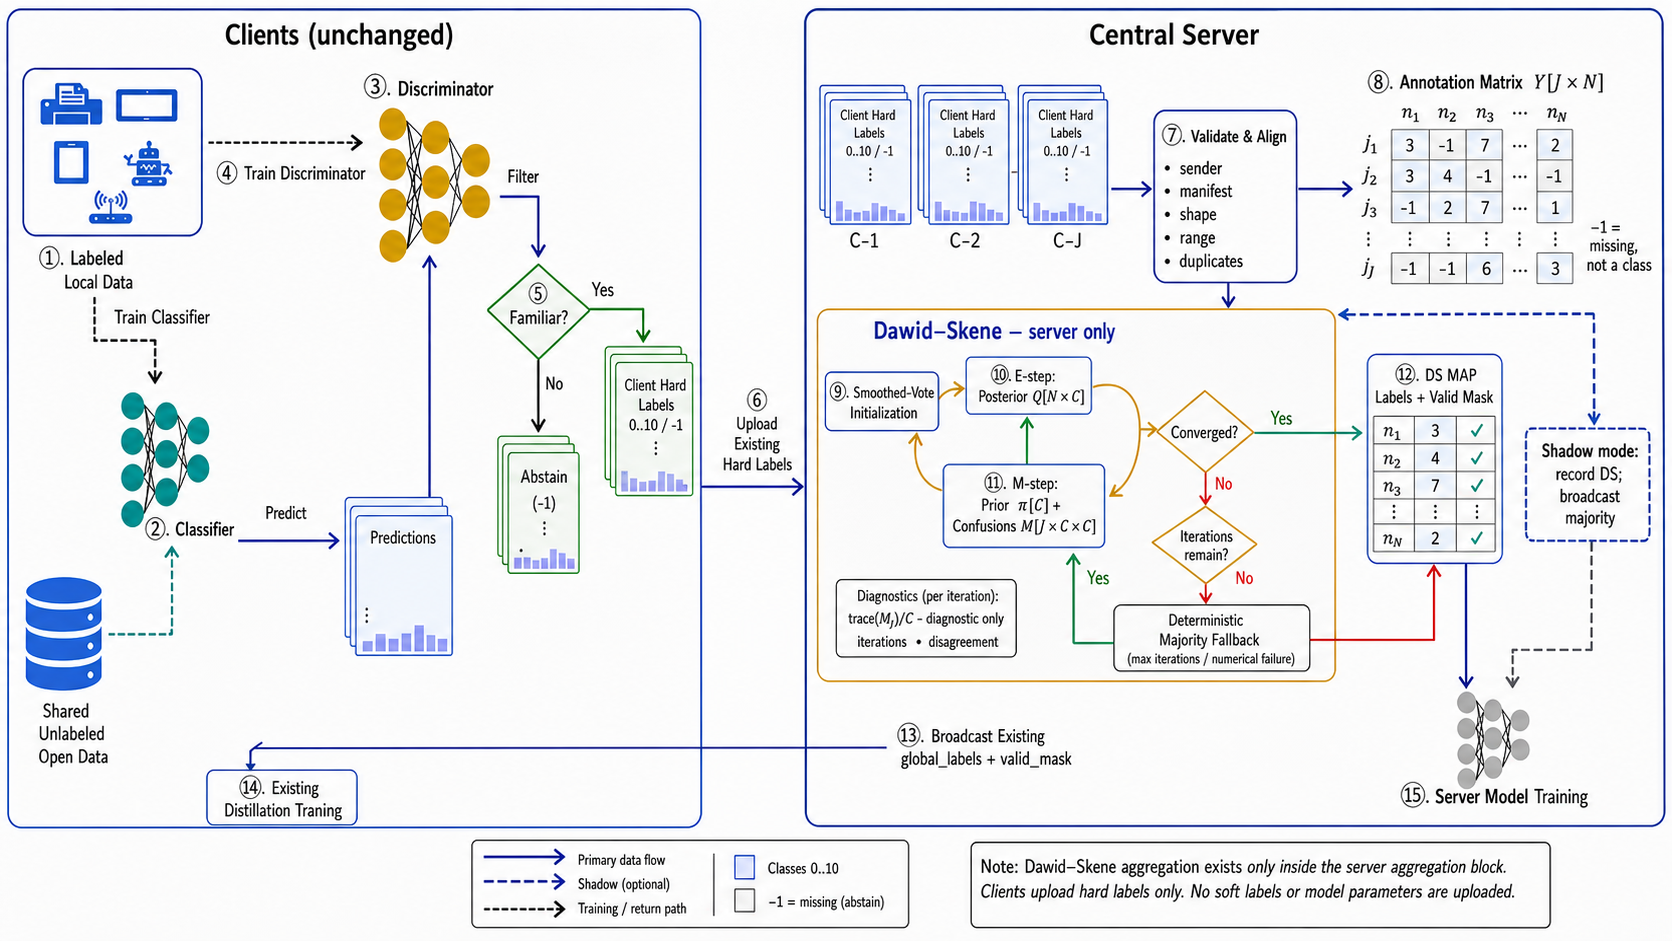
\includegraphics[width=0.97\linewidth,height=0.77\textheight,keepaspectratio]
    {DAWID_SKENE_SERVER_ARCHITECTURE.png}
  \caption{Detailed architecture. Clients are unchanged. Dawid-Skene exists only inside the
  central server aggregation block. In active mode, a successful fit supplies the hard MAP labels.
  In shadow mode, the server records the Dawid-Skene result but broadcasts majority labels. If the
  iteration limit is reached without convergence, or a numerical check fails, the majority
  fallback is used. Downstream training is not part of the Dawid-Skene loop.}
  \label{fig:architecture}
\end{figure}
\end{landscape}
\clearpage

\section{How Dawid-Skene works, without the jargon}

Majority voting asks only, ``How many clients chose each answer?'' Dawid-Skene also asks, ``Based
on the complete pattern of agreements and disagreements, which clients are informative for this
particular class?''

The server performs the following cycle independently in each round:

\begin{enumerate}
  \item \textbf{Build the table.} Put every accepted client's label vector into a stable
        client-by-sample matrix.
  \item \textbf{Ignore abstentions.} A \code{-1} entry contributes no label evidence for that
        client and sample.
  \item \textbf{Start cautiously.} Use smoothed vote proportions as the initial estimate. Smoothing
        avoids declaring any class mathematically impossible at the start.
  \item \textbf{Reconsider the samples.} Estimate the probability that each sample belongs to each
        class, using the current client confusion patterns. This is the E-step.
  \item \textbf{Reconsider the clients.} Estimate, for every eligible client and true class, how
        that client tends to label the class. This is the M-step.
  \item \textbf{Repeat safely.} Alternate the previous two steps until the regularized objective
        changes by no more than the tolerance, or the iteration limit is reached.
  \item \textbf{Choose hard labels.} For every supported sample, select the class with the largest
        posterior probability. Preserve the existing validity-mask interface.
\end{enumerate}

The estimated scalar
\[
  \text{diagnostic reliability of client }j
  = \frac{\operatorname{trace}(M_j)}{C}
\]
is stored only as a restricted diagnostic. It does not weight uploaded model parameters and it is
not sent to clients.

\subsection{Important technical safeguards in simple terms}

\begin{itemize}
  \item Calculations use 64-bit floating-point numbers and log space. This avoids tiny probability
        products becoming zero because of computer precision.
  \item Small pseudocounts are added to class and confusion counts. This prevents unsupported rows
        from becoming impossible zero-probability rows.
  \item Because pseudocount priors are active, convergence is checked using a matching regularized
        objective. Raw data likelihood is recorded separately rather than used under the wrong
        name.
  \item Vote-based initialization encourages the hidden class numbers to retain the repository's
        class meanings. It does not mathematically guarantee that label switching or a poor local
        solution can never occur.
  \item Confusion matrices are estimated again in every round in the primary study. They are not
        permanent client reputation scores. Warm start is disabled.
\end{itemize}

\section{Input rules and deterministic behavior}

The server must produce the same answer when the same valid submissions arrive in a different
order. The adapter therefore applies explicit rules:

\begin{itemize}
  \item Every label vector must have exactly $N$ entries and contain only \code{-1} or classes
        0 through $C-1$.
  \item Sender identifiers are processed in sorted order.
  \item Identical retries from one sender are accepted once and recorded as retries.
  \item If the same sender submits conflicting label vectors, that sender is rejected for the
        round and the reason is recorded.
  \item Clients below the minimum annotation count are excluded from estimation and reported.
  \item The proposed practical support gate requires at least three eligible clients. This is a
        guard, not a proof that every three-client problem is statistically identifiable.
  \item Samples with too few usable observations are not fitted or broadcast as valid.
  \item An exact class tie uses the lowest class index, preserving deterministic behavior.
\end{itemize}

\section{Safety, fallback, and shadow mode}

\subsection{When the server falls back to majority}

The proposed policy is \code{majority\_on\_failure\_or\_nonconvergence}. The server records the
reason and uses deterministic majority voting if any of the following occurs:

\begin{itemize}
  \item there are no estimable observations;
  \item fewer than the required number of clients are eligible;
  \item a prior, posterior, confusion value, likelihood, or objective becomes undefined or infinite;
  \item a probability vector does not normalize correctly;
  \item the regularized objective decreases beyond the numerical tolerance; or
  \item the maximum iteration count is reached without convergence.
\end{itemize}

Fallback keeps a round running; it does not prove that the majority answer is correct. The fallback
rate is therefore a reported outcome and a decision gate.

If no valid proposal is received at all, returning ``no update'' is unsafe because an orchestrator
can retain old arrays. The server must instead emit an explicit vector of \code{-1} labels and an
all-false validity mask. This prevents stale labels from being reused.

\subsection{Why shadow mode comes first}

In shadow mode the server computes and audits Dawid-Skene, but broadcasts majority labels. The
training trajectory therefore stays on the current majority path. This is the only live mode where
majority and Dawid-Skene see exactly the same client proposals throughout the run.

Once active Dawid-Skene labels are broadcast, client models can develop differently from the
majority arm. Later proposals are then part of the treatment effect; they should not be described
as identical. Active comparisons instead share the same initial state, seeds, scenario, code,
hardware controls, and paired run identity.

\section{Software changes}

\begin{longtable}{L{0.33\textwidth}L{0.61\textwidth}}
\caption{Planned implementation points.}\label{tab:codechanges}\\
\toprule
\textbf{File or component} & \textbf{Plain-English responsibility} \\
\midrule
\endfirsthead
\toprule
\textbf{File or component} & \textbf{Plain-English responsibility} \\
\midrule
\endhead
\bottomrule
\endfoot
\path{src/ssfl/protocols/dawid_skene.py} & New self-contained NumPy estimator. It owns the
E-step, M-step, initialization, stopping rules, invariants, result type, and failure signal. \\
\path{src/ssfl/protocols/ssfl.py} & Turn validated hard-label proposals into the stable annotation
matrix, call the selected aggregator, and return the existing aggregation result fields. \\
\path{src/ssfl/config.py} & Add resolved Dawid-Skene fields, ranges, valid mode combinations, stable
configuration hashing, and rejection of unsupported warm start. \\
\path{src/ssfl/strategies/ssfl.py} & Select majority, shadow, or active Dawid-Skene inside
\code{aggregate\_train}; guarantee explicit no-proposal output and visible fallback. \\
\path{src/ssfl/server_app.py} & Build validated options and inject a diagnostics ledger into the
strategy. Client and distillation wiring stays unchanged. \\
\path{src/ssfl/metrics.py} & Add a resume-aware aggregation diagnostics ledger. Round records are
committed atomically so failed or resumed attempts cannot duplicate or replace good records. \\
\path{src/ssfl/reporting/build_report.py} & Produce a separate feasibility comparison keyed by run
kind and aggregation mode. Extension runs cannot silently replace canonical report cells. \\
\path{tests/protocol/test_dawid_skene.py} & Add hand-computed, synthetic, missing-label,
determinism, convergence, failure, and reliability tests. \\
Existing configuration, integration, privacy, resume, and report tests & Prove unchanged payloads,
valid mode combinations, restricted audit defaults, clean resume behavior, and report separation. \\
\end{longtable}

\section{Configuration and starting values}

All settings must appear in the resolved configuration, run identity, and report. The values below
are \textbf{candidate screening values}. They are not defaults claimed by the reference paper and
they must be locked before active testing.

\begin{longtable}{L{0.36\textwidth}L{0.18\textwidth}L{0.39\textwidth}}
\caption{Complete proposed configuration dictionary.}\label{tab:hyperparameters}\\
\toprule
\textbf{Field} & \textbf{Candidate} & \textbf{Meaning in plain English} \\
\midrule
\endfirsthead
\toprule
\textbf{Field} & \textbf{Candidate} & \textbf{Meaning in plain English} \\
\midrule
\endhead
\bottomrule
\endfoot
\path{ssfl_hard_aggregation} & \path{dawid_skene_shadow} & Server aggregation mode:
majority, shadow, or active Dawid-Skene. \\
\path{dawid_skene_max_iterations} & 100 & Hard ceiling on E/M cycles. \\
\path{dawid_skene_min_iterations} & 2 & Prevent a convergence declaration at the starting point. \\
\path{dawid_skene_tolerance} & $10^{-6}$ & Relative regularized-objective change required to stop. \\
\path{dawid_skene_initialization} & \path{smoothed_votes} & Starting estimate; screening also
tests one-hot majority and a near-diagonal confusion start. \\
\path{dawid_skene_initialization_pseudocount} & 0.01 & Small starting mass for every class. \\
\path{dawid_skene_initial_diagonal_probability} & 0.9 & Used only in the near-diagonal
initialization sensitivity arm. \\
\path{dawid_skene_confusion_pseudocount} & 0.1 & Prevent zero entries in confusion rows. \\
\path{dawid_skene_class_prior_pseudocount} & 1.0 & Prevent zero or collapsed initial class priors. \\
\path{dawid_skene_min_item_annotations} & 1 & Minimum usable client labels for a sample. \\
\path{dawid_skene_min_client_annotations} & 1 & Minimum submitted labels for a client to be fitted. \\
\path{dawid_skene_min_clients} & 3 & Practical support gate before fitting. \\
\path{dawid_skene_posterior_threshold} & 0.0 & Primary comparison does not gain by rejecting
lower-confidence samples. \\
\path{dawid_skene_warm_start} & \path{false} & Required in the first implementation. Reject
\code{true} until stable logical identity and resume semantics exist. \\
\path{dawid_skene_damping} & 1.0 & Use the full M-step update in the primary study. \\
\path{dawid_skene_epsilon} & $10^{-12}$ & Log-space clipping safeguard. \\
\path{dawid_skene_internal_dtype} & \path{float64} & Numerical precision used by the estimator. \\
\path{dawid_skene_failure_policy} & \path{majority_on_failure_or_nonconvergence} & Visible
continuity behavior for invalid or capped fits. \\
\path{dawid_skene_save_annotations} & \path{false} & Raw client-by-sample storage is off by default. \\
\path{dawid_skene_full_audit_rounds} & 1, 10, 50 & Full posterior/confusion audits for the
50-round profile; a 200-round profile can add 100, 150, and 200. \\
\end{longtable}

\section{Feasibility and expected cost}

The estimator is small enough in memory. Runtime is the main engineering uncertainty.

\begin{table}[htbp]
\centering
\caption{Largest-scenario compact memory estimates.}
\begin{tabularx}{\textwidth}{Y L{0.25\textwidth} L{0.22\textwidth}}
\toprule
\textbf{Array} & \textbf{Shape and type} & \textbf{Approximate size} \\
\midrule
Annotations & $89 \times 8{,}900$ bytes & 0.76 MiB \\
Posterior probabilities & $8{,}900 \times 11$ float64 & 0.75 MiB \\
Client confusion matrices & $89 \times 11 \times 11$ float64 & 0.08 MiB \\
Naive temporary to avoid & $89 \times 8{,}900 \times 11$ float64 & 66.5 MiB \\
\bottomrule
\end{tabularx}
\end{table}

One full iteration has both an E-step and an M-step. The approximate contribution counts are:

\begin{itemize}
  \item 27-client scenario: 5.29 million per full iteration, or about 529 million at 100 iterations;
  \item 89-client scenarios: 17.42 million per full iteration, or about 1.74 billion at 100 iterations.
\end{itemize}

The implementation must use indexed gathers, counting operations, and optional chunking rather than
materializing the naive three-dimensional temporary. Early stopping should avoid using the ceiling
on easy rounds. A 100-iteration live ceiling is the starting proposal; 50, 100, and 500 are screened
offline. Real wall time, peak memory, and audit-writing time must be measured separately.

\section{The controlled experiment}

The purpose of the experiment is not to show that a complicated method can run. It is to establish
whether the server-side aggregation change improves labels and downstream learning under a fair,
repeatable comparison.

\begin{table}[htbp]
\centering
\caption{Staged experiment plan. Phase 4 is not part of the primary decision.}
\small
\begin{tabularx}{\textwidth}{L{0.11\textwidth}L{0.18\textwidth}Y L{0.15\textwidth}}
\toprule
\textbf{Phase} & \textbf{Scale} & \textbf{Purpose and rule} & \textbf{Federated runs} \\
\midrule
0: gates & Local fixtures and scenario-sized benchmarks & Hand-computed mathematics, synthetic
clients, missingness, ordering, failure, determinism, latency, and memory. & 0 \\
1: shadow & 3 scenarios, seed 2023, 50 rounds & Majority stays active. Compute Dawid-Skene on the
same proposals. Screen 12 declared settings on development and check one winner once on validation. & 3 \\
2: pilot & 3 scenarios, seeds 2023--2025, 50 rounds & Nine matched majority/Dawid-Skene pairs.
Lock settings before this phase. & 18 \\
3: confirmation & 3 scenarios, seeds 2026--2035, 200 rounds & Thirty matched pairs with no setting
changes after the pilot. Seeds are new and independent of screening. & 60 \\
4: later ablations & Only after confirmation & Test filtering, evidence thresholds, confidence
thresholds, damping, stable-identity warm start, tie-breaks, and soft posterior distillation as
separate questions. & Not in primary plan \\
\bottomrule
\end{tabularx}
\end{table}

The plan through confirmation contains 81 federated runs: 3 shadow runs, 18 pilot runs, and 60
confirmation runs. This excludes local fixtures, benchmarks, and later ablations.

\subsection{Locked dataset and training controls}

\begin{longtable}{L{0.29\textwidth}L{0.65\textwidth}}
\toprule
\textbf{Control} & \textbf{Locked value or rule} \\
\midrule
\endfirsthead
\toprule
\textbf{Control} & \textbf{Locked value or rule} \\
\midrule
\endhead
\bottomrule
\endfoot
Dataset identity & Prepared N-BaIoT manifest; hash
\texttt{54023e3de197d9dc16f50a89425d5c44}\newline
\texttt{bb594486210aacf16ecaa8cccc86ba65}. \\
Split sizes & 8,900 shared open samples; 62,300 private samples; 17,800 test samples. \\
Classes & 11. Open-set counts are 900 each for classes 0--5 and 700 each for classes 6--10. \\
Scenarios & 1, 2, and 3, with 27, 89, and 89 structural clients. \\
Participation & All structural clients per round, with actual participation, retries, and failures recorded. \\
Model and training & CNN; persistent model weights; fresh Adam per task; learning rate $10^{-4}$;
five local epochs; batch size 80. \\
Filtering & Discriminator enabled with the median threshold in the primary comparison. \\
Labels & Existing hard int8 labels and abstention semantics. \\
Initialization & Same seeded model checkpoints inside every matched pair. \\
Infrastructure & Same commit, dependency lock, drivers, hardware, deterministic settings, GPU
allocation, and concurrency. Run order is randomized or interleaved. \\
Run identity & Explicit scenario-seed pair ID, all random seeds, node-to-logical-client mapping,
checkpoint state, and a clean committed worktree. \\
Only active difference & The server hard-label aggregation setting and its locked Dawid-Skene options. \\
\end{longtable}

\subsection{Screening without hidden tuning freedom}

The 12 candidate configurations and the exact development/validation split are declared before
scores are read. Development uses scenario 1, seed 2023, rounds 1, 5, 10, 15, 20, and 25, on hash
buckets 0--1 of the open items. Validation uses later scenario-1 rounds and selected rounds from
scenarios 2 and 3, on hash buckets 2--4. Test accuracy from active runs is never a tuning signal.

The screen changes one setting at a time: iteration ceiling, tolerance, initialization family,
initialization smoothing, confusion smoothing, or class-prior smoothing. Minimum evidence,
posterior threshold, damping, and warm start remain fixed. The winner is selected by development
macro-F1, then worst-class recall, runtime, lower iteration ceiling, and finally configuration ID.
Any setting that fails or falls back is ineligible. If the one-time validation check misses the
shadow gate, the experiment stops or a new study is preregistered; validation is not reused for
retuning.

\section{What will be measured}

\subsection{Label quality, offline only}

After a run, a separate evaluator may join outputs to sealed open-set truth. Live aggregation and
training cannot import those labels. The offline report includes:

\begin{itemize}
  \item label accuracy and macro, micro, and weighted precision, recall, and F1;
  \item per-class confusion, recall, F1, and valid coverage;
  \item matched-coverage comparisons so one method cannot win merely by rejecting more samples;
  \item disagreements, corrected errors, newly introduced errors, and net corrections;
  \item tie and non-tie subsets;
  \item posterior negative log-likelihood, Brier score, entropy, and 15-bin equal-frequency
        calibration error on estimable items only;
  \item predicted class balance, annotation support, diagonal dominance, and estimated versus
        audit-only empirical client confusion.
\end{itemize}

\subsection{Downstream model quality}

The two co-primary outcomes are the mean server macro-F1 and mean server accuracy over the final 10
rounds. Accuracy matches the reference paper's convention; macro-F1 protects against a model that
looks good overall while failing a minority class.

Secondary outcomes include worst-class recall, per-class F1, final and best scores, learning-curve
area, raw and normalized confusion matrices, loss, valid-label rate, and time to 50\% and 75\%
accuracy. Runs that never reach a target are right-censored rather than assigned a fake round 200
achievement.

A \textbf{new class collapse} means that a supported class has Dawid-Skene final-10 recall below
5\% while its matched majority run retains at least 20\% recall. Every class below 5\% in either arm
is still disclosed.

\subsection{Statistical unit}

An item and a training round are not independent experiments. First calculate the
Dawid-Skene-minus-majority final-10 difference inside each scenario-seed pair. Report scenarios
separately. For the overall confirmation result, average the three scenario differences within each
seed and treat the 10 seeds as independent blocks. Report paired intervals and the declared
one-sided exact paired tests, while acknowledging the limited power of 10 blocks.

Every assigned Dawid-Skene round remains in the Dawid-Skene arm even if it falls back to majority.
This is the intention-to-treat analysis. Algorithmic failures are not replaced with better seeds.
An unresolved missing matched pair is disclosed and blocks adoption.

\subsection{Engineering behavior}

Record iterations, stop reason, raw likelihood, regularized-objective history, fallback reason,
latency, peak memory, temporary allocation, audit storage, participation, and support. Confirm exact
equality of network tensor names, data types, shapes, and logical byte counts. Serialized bytes are
reported separately; they can vary when active training changes existing values, but no new
Dawid-Skene payload is allowed.

\section{Decision gates}

These are proposed preregistration thresholds, not observed results or guarantees.

\begin{longtable}{L{0.24\textwidth}L{0.70\textwidth}}
\caption{Promotion, adoption, and stopping rules.}\label{tab:gates}\\
\toprule
\textbf{Decision} & \textbf{Required evidence} \\
\midrule
\endfirsthead
\toprule
\textbf{Decision} & \textbf{Required evidence} \\
\midrule
\endhead
\bottomrule
\endfoot
Shadow to active pilot & Finite, invariant-valid output every round; at least 95\% convergence; no
unexplained objective decrease; positive net corrections in every scenario; at least +1 \pp{}
matched-coverage macro-F1; at least +5 \pp{} on the targeted problem-class subset; scenario-89 p95
compute time below both 10\% of round time and 5 seconds; zero logical byte-count change; no new
wire field; any serialized-byte difference below 1\% and explained. \\
Pilot to confirmation & Mean paired final-10 macro-F1 at least +1 \pp{}; accuracy non-inferior
within -0.5 \pp{}; no scenario loses more than 1 macro-F1 point; at least 8 of 9 pairs improve
macro-F1; worst-class recall improves with no new class collapse; fallback below 1\%; wall-clock
overhead below 10\%; no protocol payload change. \\
Adopt after confirmation & Ten seed-block macro-F1 differences average at least +1 \pp{} and pass
the declared one-sided test at $\alpha=0.05$; accuracy passes the -0.5 \pp{} non-inferiority test;
both co-primary conditions pass; all runs are disclosed; no scenario loses more than 1 point; no
new class collapse, privacy breach, protocol increase, or systems regression. \\
Stop or redesign & Label switching, class collapse, gains obtained mainly by rejecting samples,
worse non-tie decisions, frequent sparse or numerical fallback, use of sealed labels in the live
path, gains confined to one seed or scenario, unacceptable sensitive-profile risk, or excessive
runtime after optimization. \\
\end{longtable}

\section{Privacy, audit, and reproducibility}

Keeping the network payload unchanged does not remove every privacy concern. Dawid-Skene can create
a per-client profile of class-specific error patterns. Those profiles and the raw annotation matrix
are more sensitive than aggregate vote totals.

The proposed controls are:

\begin{itemize}
  \item raw annotation storage is off by default and allowed only for restricted Phase-1 shadow audits;
  \item scenario 1 retains rounds 1, 5, 10, 15, 20, 25, 30, 35, 40, 45, and 50; scenarios 2 and 3
        retain rounds 1, 10, 25, 35, and 50, exactly matching the screen;
  \item sender IDs are replaced by a run-scoped HMAC pseudonym before storage; this is
        pseudonymization, not complete anonymization;
  \item sensitive files use compressed, encrypted, owner-only storage with directory mode 0700;
  \item raw annotations and the HMAC key are deleted within 30 days after Phase-1 settings are locked;
  \item per-client files remain outside the general report bundle;
  \item truth-based quality evaluation is offline and cannot feed back into an active run;
  \item attempt-local files are promoted atomically only after the round checkpoint commits;
        resume truncates rows after the checkpoint and discards incomplete attempt files.
\end{itemize}

\begin{table}[htbp]
\centering
\caption{New or extended experiment artifacts.}
\begin{tabularx}{\textwidth}{L{0.34\textwidth}Y}
\toprule
\textbf{Artifact} & \textbf{Contents and access} \\
\midrule
\path{aggregation_metrics.parquet} & Round-level mode, support, convergence, iterations, raw
likelihood, objective, entropy, timing, fallback, and disagreement. \\
\path{dawid_skene_clients.parquet} & Restricted client reliability, support, and confusion
summaries; excluded from general telemetry and report bundles. \\
\path{aggregation_quality.parquet} & Offline truth-based majority/Dawid-Skene comparisons; never
read by training. \\
\path{aggregation_audit/*.npz} & Existing vote/label/mask data plus selected-round posterior,
prior, confusion, and optionally restricted annotations. \\
\bottomrule
\end{tabularx}
\end{table}

Every run also records its resolved configuration, manifest hash, all seeds, scenario, client
mapping, participation, retries, code revision, dependency versions, hardware, checkpoints, and
dirty-worktree state. Confirmation requires a clean committed worktree.

\section{Risks and limitations}

\begin{longtable}{L{0.26\textwidth}L{0.30\textwidth}L{0.36\textwidth}}
\caption{What can go wrong and how it will be detected.}\label{tab:risks}\\
\toprule
\textbf{Risk} & \textbf{Why it matters} & \textbf{Control or diagnostic} \\
\midrule
\endfirsthead
\toprule
\textbf{Risk} & \textbf{Why it matters} & \textbf{Control or diagnostic} \\
\midrule
\endhead
\bottomrule
\endfoot
Clients make correlated errors & Dawid-Skene assumes errors are conditionally independent once the
true class is known. Similar models can make the posterior overconfident. & Calibration, entropy,
synthetic correlated-error tests, and cautious interpretation of confidence. \\
Abstention is not random & The discriminator is more likely to abstain on particular samples and
classes, which can bias confusion estimates. & Treat abstention as missing, report class/client
support, and test alternate filter modes only after the primary study. \\
Specialist clients lack some classes & A confusion row can have little real evidence. & Pseudocounts,
minimum support, effective client-by-class support, and excluded-client reporting. \\
Many clients make the same mistake & Agreement without gold truth cannot expose a unanimous
correlated error. & State the limitation, examine offline truth only after runs, and never claim
consensus is ground truth. \\
Hidden labels switch meaning & A latent class can move away from the repository's semantic class
index. & Vote-anchored initialization, diagonal-dominance diagnostics, synthetic tests, shadow mode,
and no-go on detected switching. \\
Slow server rounds & Repeated E/M passes can dominate 200-round experiments. & Early stopping,
iteration cap, indexed operations, chunking, separate benchmarks, and hard latency gates. \\
Sensitive client profiles & Confusion matrices can act like quality or behavior profiles. & Default
off, pseudonymization, restricted encrypted storage, access separation, deletion, and privacy review. \\
Report collision & An extension could silently replace an existing canonical result. & Key reports
by run kind and aggregation mode and test that canonical cells cannot be superseded. \\
\end{longtable}

\section{Verification plan}

Before any active experiment, the implementation must pass the following groups of tests.

\subsection{Mathematics and estimator behavior}

\begin{itemize}
  \item one hand-derived E-step and M-step;
  \item perfect, unreliable, adversarial, imbalanced, sparse, and missing-label synthetic clients;
  \item finite and normalized priors, posteriors, and confusion rows;
  \item non-decreasing regularized objective within numerical tolerance;
  \item absent classes, all-abstain samples, exact MAP ties, and one-client inputs;
  \item forced numerical failure and iteration-cap fallback;
  \item synthetic reliability rankings and label-alignment stress tests.
\end{itemize}

\subsection{Protocol, configuration, and determinism}

\begin{itemize}
  \item identical output under every valid sender order;
  \item deterministic handling of identical and conflicting duplicate replies;
  \item strict ranges and valid hard-label mode combinations;
  \item rejected warm start in the first implementation;
  \item every option changes the resolved run identity;
  \item canonical majority behavior remains unchanged;
  \item extension runs cannot populate canonical report cells.
\end{itemize}

\subsection{Integration, privacy, resume, and performance}

\begin{itemize}
  \item two-round CPU smoke runs in shadow and active modes;
  \item shadow output and valid fallback output match majority for valid unique-sender batches;
  \item clients consume only the existing labels and mask;
  \item no new payload field or logical byte count;
  \item live code cannot read sealed truth labels;
  \item restricted files are absent by default;
  \item resume reproduces committed output and removes incomplete diagnostics;
  \item scenario-sized 27- and 89-client latency and peak-memory benchmarks.
\end{itemize}

\section{Implementation sequence}

If the server-side scope and experimental defaults are approved, the safest order of work is:

\begin{enumerate}
  \item add validated configuration fields while keeping majority as the default;
  \item implement the pure Dawid-Skene estimator and its tagged success/failure result;
  \item add mathematical, synthetic, missing-data, and determinism unit tests;
  \item add the proposal-to-annotation adapter and preserve the existing result contract;
  \item add shadow and active strategy selection with explicit all-abstain no-proposal output;
  \item add the resume-safe diagnostics ledger and restricted audit controls;
  \item add the offline truth evaluator and report identity separation;
  \item run protocol, privacy, resume, and payload-equivalence tests;
  \item benchmark 27- and 89-client scenarios and optimize indexed operations if needed;
  \item run Phase 1 shadow screening, lock settings, and apply the preregistered gate;
  \item proceed to the paired pilot and confirmation only when each prior gate passes.
\end{enumerate}

No production implementation should be called complete merely because the estimator returns labels.
Configuration, failure behavior, audits, offline evaluation, reporting separation, privacy controls,
and tests are part of the required change.

\section{Decisions and recommended defaults}

The server-only scope is now the working assumption. The remaining approvals have recommended
defaults:

\begin{enumerate}
  \item \textbf{Abstention:} keep \code{-1} as a missing observation. Requiring every client to label
        every sample would change the current protocol and filter behavior.
  \item \textbf{Primary outcomes:} use final-10 macro-F1 and accuracy together. Macro-F1 protects
        classes; accuracy preserves comparability with the paper.
  \item \textbf{Sensitive audit:} allow raw annotations only for the declared Phase-1 rounds under
        owner-only encrypted storage and 30-day deletion. If that storage is unavailable, compute
        all screen variants online and do not save raw annotations.
  \item \textbf{Compute budget:} authorize one phase at a time: three shadow runs, then 18 pilot
        runs, then 60 confirmation runs only if the earlier gates pass.
\end{enumerate}

\appendix

\section{Plain-English server pseudocode}

\begin{lstlisting}[style=plainpseudo]
For each server round:
  collect and validate the existing hard-label proposals

  if no valid proposal exists:
      broadcast all -1 labels and an all-false valid mask
      record "no proposals"
      stop this aggregation

  if the configured mode is majority:
      run the unchanged majority aggregator
      broadcast its existing labels and mask
      stop this aggregation

  group all replies by sender
  accept one copy of identical retries
  reject a sender if its duplicate payloads conflict
  sort accepted senders and build Y[client, sample]
  treat -1 cells as missing observations

  compute the deterministic majority result for fallback

  if fewer than the required clients or items have support:
      record the support failure
      broadcast the majority result
      stop this aggregation

  initialize class probabilities from smoothed votes
  initialize the class prior and client confusion matrices

  repeat up to max_iterations:
      E-step: estimate class probabilities for every usable item
      record raw likelihood and the regularized objective
      check all finite/normalization/monotonicity rules

      if the regularized objective has converged:
          mark success and stop repeating

      if another iteration remains:
          M-step: update the class prior and client confusion matrices

  if the fit failed or hit the cap without convergence:
      record the reason
      broadcast the majority result
  else if mode is shadow:
      save Dawid-Skene diagnostics
      broadcast the majority result
  else:
      choose the highest-posterior class for each supported item
      broadcast those hard labels and the existing valid mask

  never broadcast posterior, confusion, or reliability arrays
  commit diagnostics only after the round checkpoint commits
\end{lstlisting}

\section{The 12-setting shadow screen}

\begin{longtable}{L{0.15\textwidth}L{0.77\textwidth}}
\toprule
\textbf{ID} & \textbf{Single change from the candidate configuration} \\
\midrule
\endfirsthead
\toprule
\textbf{ID} & \textbf{Single change from the candidate configuration} \\
\midrule
\endhead
\bottomrule
\endfoot
DS-00 & Candidate: 100 iterations, tolerance $10^{-6}$, smoothed votes, initialization
pseudocount 0.01, confusion pseudocount 0.1, class-prior pseudocount 1.0. \\
DS-01 & Maximum iterations 50. \\
DS-02 & Maximum iterations 500. \\
DS-03 & Tolerance $10^{-4}$. \\
DS-04 & Tolerance $10^{-8}$. \\
DS-05 & One-hot majority initialization. \\
DS-06 & Near-diagonal confusion initialization with diagonal probability 0.9. \\
DS-07 & Initialization pseudocount 0.001. \\
DS-08 & Initialization pseudocount 0.1. \\
DS-09 & Confusion pseudocount 0.01. \\
DS-10 & Confusion pseudocount 1.0. \\
DS-11 & Class-prior pseudocount 0.1. \\
\end{longtable}

All 12 keep minimum item annotations 1, minimum client annotations 1, minimum clients 3,
posterior threshold 0.0, damping 1.0, and warm start false. Every attempted result is published.

\section{Glossary}

\begin{longtable}{L{0.25\textwidth}L{0.69\textwidth}}
\toprule
\textbf{Term} & \textbf{Meaning} \\
\midrule
\endfirsthead
\toprule
\textbf{Term} & \textbf{Meaning} \\
\midrule
\endhead
\bottomrule
\endfoot
Abstention & A client provides no label for one sample. Stored as \code{-1} and treated as missing. \\
Annotation & One client's proposed label for one shared sample. \\
Class prior & The estimated share of usable samples belonging to each class. \\
Confusion matrix & A class-by-class table describing which labels a client tends to output for
each hidden true class. \\
Convergence & The iterative estimates have changed by no more than the declared tolerance. \\
Damping & Blending a new update with the previous update instead of replacing it fully. \\
E-step & Re-estimate sample class probabilities using current client error patterns. \\
Fallback & Use deterministic majority when Dawid-Skene cannot finish safely. \\
Hard label & One selected class number rather than a full probability vector. \\
Latent label & The unknown class that the server is trying to estimate. \\
Log space & A numerically stable way to add log probabilities instead of multiplying tiny numbers. \\
M-step & Re-estimate the class prior and client confusion matrices using current sample probabilities. \\
Macro-F1 & Calculate F1 for every class and average the classes equally. \\
Posterior probability & The estimated probability of a class after considering the submitted labels. \\
Pseudocount & A small artificial count that prevents zero probabilities and stabilizes sparse rows. \\
Shadow mode & Compute and record Dawid-Skene while continuing to broadcast majority labels. \\
Valid mask & A Boolean vector telling downstream code which global labels may be used. \\
Warm start & Start a new round from a previous round's Dawid-Skene parameters. Disabled here. \\
\end{longtable}

\section{Reference and scope note}

The mathematical reference is J. Dong, R. Zhu, X. Shang, and J.-H. Xue,
``Dawid-Skene-model-based label-noise mitigation for federated learning,''
\emph{Information Sciences}, volume 745, article 123425, 2026,
\href{https://doi.org/10.1016/j.ins.2026.123425}{doi:10.1016/j.ins.2026.123425}.

That paper's FedDS workflow uploads client model parameters, runs the client models on public data
at the server, estimates reliability, and uses reliability to weight model aggregation. This report
does not propose that protocol. It proposes Dawid-Skene only at the existing server hard-label
aggregation seam. Operational choices that the paper does not fully prescribe here - initialization,
smoothing, abstention handling, stopping, warm start, fallback, and audit behavior - are explicit
experimental settings rather than hidden assumptions.

\vfill
\begin{center}
  \color{DarkGray}\small End of report
\end{center}

\end{document}
